\section{Data Collection}
\label{res-met:data-collection}

% \subsection{Techniques of data collection}

% \fbox{
%     \begin{minipage}[htb]{0.9\textwidth}
%         \vspace{0.3cm}
                
%         \colorbox{gray!30}{% create a colored box
%             \makebox[0.975\textwidth][l]{% center the text on the page
%                 \ \ \textbf{Further Writing}
%             }
%         }

%         \vspace{0.1cm}
        
%         \begin{itemize}
%             \item Presenting the four major philosophical frameworks possible to follow during a qualitative research.
%             \item Describing my position, situating between interpretive and critical frameworks.

%         \end{itemize}

%         \vspace{0.25cm}
        
%     \end{minipage}
% }

In this research, I collected data using four techniques: interviews, questionnaires, document surveys, and observational notes. For collecting interview data, I adopted a sampling strategy (Section \ref{res-met-ss:sampling-strategy}) using the Lorenz Curve (Section \ref{res-meth-ss:lorenz}) as an auxiliary instrument to classify students in a class.

\begin{table}[ht]
\caption{Epistemological perspectives from their main purposes, types of research, and perceptions of reality.}
\label{tbl:epist-perspectives}
\centering
\rowcolors{1}{}{lightgray}
\begin{tabular}{
    p{1.9cm}|
    m{2.6cm}|
    m{2.7cm}|
    m{2.5cm}|
    m{2.8cm}
}
    \hline
    &
    \multicolumn{4}{c}{
        \textbf{Epistemological Perspectives}
    } \\
    \hline
    &
    \textbf{Positivist/ Postpositivist} & 
    \textbf{Interpretive/ Constructivist} & 
    \textbf{Critical} &
    \textbf{Postmodern/ Poststructural}
    \\
    \hline
    \textbf{Purpose} &
    Predict, control, generalize & 
    Describe, understand, interpret & 
    Change, emancipate, empower & 
    Deconstruct, problematize, question, interrupt
    \\
    \hline
    \textbf{Types} &
    Experimental, survey, quasi- experimental &
    Phenomenology, ethnography, hermeneutic, grounded theory, naturalistic / qualitative &
    Neo-Marxist, feminist, participatory action research (PAR), critical race theory, critical ethnography &
    Postcolonial, poststructural, postmodern, queer theory\\
    \hline
    \textbf{Reality} &
    Objective, external, out there &
    Multiple \mbox{realities} \mbox{(interpretations)}, context-bound &
    Multiple realities (interpretations) situated in political, social, cultural contexts (one reality is privileged) &
    Questions assumption that there is a place where a reality resides: “Is there a there there?”\\
    \hline

    % \multicolumn{1}{c}{
    %     \textbf{\#}
    % } &
    % \multicolumn{1}{c}{
    %     \textbf{Principle}
    % } &
    % \multicolumn{1}{c}{
    %     \textbf{Relation to SDL}
    % } \\
    % \hline     
    % 1 &
    % Problem(s) at the core of the educational proposal. &
    % -\\
    % 2 &
    % Learner as the owner of the problem. &
    % Weakly\\
    % 3 &
    % Authenticity of the problem or task. &
    % -\\
    % 4 &
    % Authenticity of the learning environment. &
    % -\\
    % 5 &
    % Learner drives the problem-solving process. &
    % Strongly\\
    % 6 &
    % Complexity of the problem or task. &
    % -\\
    % 7 &
    % Learners test ideas against alternative views and contexts. &
    % Strongly\\
    % 8 &
    % Reflection on the content and process learned.
    % Strongly \\
    % 9 &
    % Collaboration and multidirectional learning. &
    % Strongly\\
    % 10 &
    % Continuous assessment. &
    % -\\
\end{tabular}

  \par\medskip\ABNTEXfontereduzida\selectfont\textbf{Source:} Adapted from \citeonline[p.~12]{merriam:2016-whatIs}. \par\medskip
\end{table}

\subsection{Sampling strategy}
\label{res-met-ss:sampling-strategy}

When we use the expression "sample" in qualitative research, it is also necessary to make additional considerations (similar to in Section \ref{res-met-ss:transferability}). \citeonline[p.~18]{merriam:2016-whatIs} assert that:
\begin{citacao}
    “Sample selection in qualitative research is usually (but not always) nonrandom, purposeful, and small, as opposed to larger, more random sampling in quantitative research”.
\end{citacao}
The underlying principle is to guarantee the condition to choose the more informative and available sample (justifying the choice intentionality) in a smaller quantity (allowing a thick description).

% \fbox{
%     \begin{minipage}[htb]{0.9\textwidth}
%         \vspace{0.3cm}
                
%         \colorbox{gray!30}{% create a colored box
%             \makebox[0.975\textwidth][l]{% center the text on the page
%                 \ \ \textbf{Further Writing}
%             }
%         }

%         \vspace{0.1cm}
        
%         \begin{itemize}
%             \item Introducing with \citeonline[p.~18]{merriam:2016-whatIs} quotation that assert that:
%             \begin{citacao}
%                 “Sample selection in qualitative research is usually (but not always) nonrandom, purposeful, and small, as opposed to larger, more random sampling in quantitative research”.
%             \end{citacao}
%             \item Complementing this quotation.
%         \end{itemize}

%         \vspace{0.25cm}
        
%     \end{minipage}
% }

%\vspace{0.5cm}

I used in this research the comparison-focused sampling strategy. This strategy “looks in depth at the significant similarities and differences between cases and the factors that explain those differences” \cite[p.~418]{patton:2015}. There is no purpose in representing the population perfectly as a whole. The aim is to learn from unusual conditions relevant to understanding a given phenomenon better.

There are many ways to conduct comparison-focused sampling. It is possible to choose clear outliers in the population (extreme case sampling) or investigate the characteristics present in "success cases" (best case sampling), for instance. I used intensity sampling, which involves “the same logic as extreme case sampling but with less emphasis on the extremes” \cite[p.~422]{patton:2015}.

The idea, in this research, is to choose participants that consist of information-rich cases that manifest the capability diversity in the classroom. This difference needs to be intense but not extreme. There are cases where extreme sampling is the best choice, but “extreme or deviant cases may be so unusual as to distort the manifestation of the phenomenon of interest” \cite[p.~422]{patton:2015}. To help me to access the capability diversity, I used the Lorenz curve.

\subsection{Lorenz Curve}
\label{res-meth-ss:lorenz}

To help in my sampling strategy, I adopted the Lorenz curve to classify the classroom from the \acrfull{HPCI} of each student. Originally, this curve “plots the percentage of total income earned by various portions of the population when the population is ordered by the size of their incomes” \cite{gastwirth:1971}. But it helps the computation of several indexes to measure social inequalities, including under educational perspectives \cite{thomas:2003}. It assists us to visualize the accumulated distribution of a certain kind of quantity in a population. 

I used the Lorenz curve to focus on the income variable to serve as an estimator for ordering students according to their \acrfull{SES}. It is true there are other ways more robust to indicate \gls{SES} like the scholarship-occupation-income triad proposed by \citeonline[p.~11]{alves:2009}. But my idea is not to classify students with excessive rigor in relation to their \gls{SES}. As this context is in a developing country, the Lorenz curve from the \gls{HPCI} was enough to divide the space into four groups to guide my sampling strategy. I will present by an example the plot of the Lorenz curve aiming to help choosing students during data collection.

Imagine that a classroom of eight students (Table \ref{tbl:classroom-dist}) has the following distribution of \gls{HPCI} in Brazilian Real (R\$). We can display these values in a sorted way, according to Figure \ref{fig:income-example}. The blue line in this figure would represent the ideal value for all students (R\$ 1,406.25), if we desire income equality, for instance. From this reference, there is an unequal distribution due to the two extreme values in this group (R\$ 500.00 and R\$ 3,500.00). 

\begin{table}[ht]
\caption{Value distribution of the HPCI of a hypothetical classroom.}
\label{tbl:classroom-dist}
\centering
\rowcolors{1}{}{lightgray}
\begin{tabular}{
    m{2.6cm}|
    m{2.7cm}|
    m{2.5cm}|
    m{2.8cm}
}
    \hline
    R\$ 500.00 &
    R\$ 2,000.00 &
    R\$ 800.00 &
    R\$ 1,500.00 \\

    R\$ 1,000.00 &
    R\$ 750.00 &
    R\$ 3,500.00 &
    R\$ 1,200.00\\
    \hline
    
\end{tabular}

  \par\medskip\ABNTEXfontereduzida\selectfont\textbf{Source:} Created by the author (2024). \par\medskip
\end{table}

\begin{figure}[ht!]
\centering

\caption{\textmd{Chart of the sorted income distribution of Table \ref{tbl:classroom-dist} values. The red lines mark both maximum and minimum values. The blue line marks the average value.}}
\label{fig:income-example}
\fcolorbox{gray}{white}{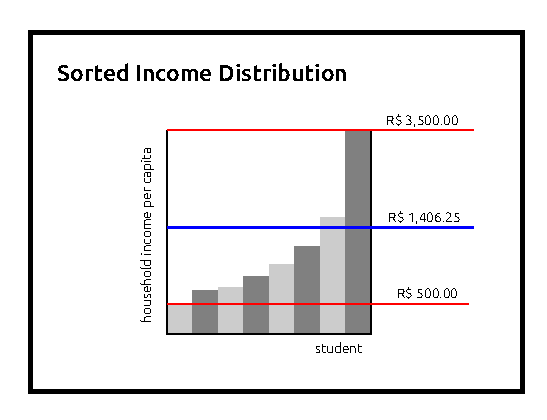
\includegraphics[width=0.9\textwidth]{images/chapter-06/income-example.pdf}}

\par\medskip\ABNTEXfontereduzida\selectfont\textbf{Source:} Created by the author (2024).
\end{figure}

\begin{figure}[ht!]
\centering

\caption{\textmd{Chart of the Lorenz curve of Table \ref{tbl:classroom-dist} values. The red line marks the maximum percentage value. The blue line represents the ideal one.}}
\label{fig:lorenz-curve-example}
\fcolorbox{gray}{white}{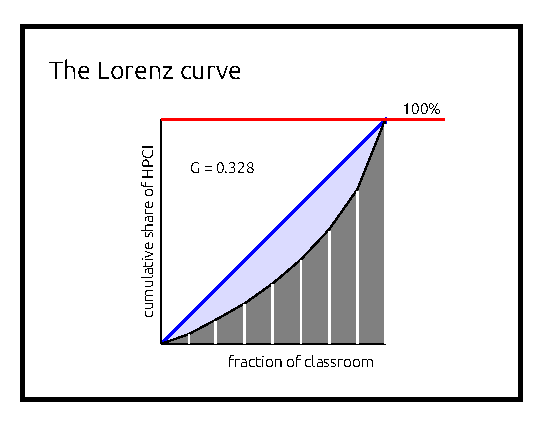
\includegraphics[width=0.9\textwidth]{images/chapter-06/lorenz-example.pdf}}

\par\medskip\ABNTEXfontereduzida\selectfont\textbf{Source:} Created by the author (2024).
\end{figure}

It is possible to see there is an inequality from Figure \ref{fig:income-example}. But if I need to compare this classroom inequality to inequalities of other people groups, it recommends normalizing all values. The Lorenz curve makes it through two steps: (i) using as normalizing reference the sum percentage of all resources (in this case, \gls{HPCI}), and (ii) working with the accumulated values of resources instead of the corresponding one of each individual. Figure \ref{fig:lorenz-curve-example} plots the Lorenz curve with the Table \ref{tbl:classroom-dist} values. 

An interesting possibility when we use the Lorenz curve is to compute the \gls{GI} \cite{farris:2010}. In this example, the \gls{GI} is 0.328\footnote{Thanks to Buck Shlegeris for opening her JavaScript code to compute Gini Index at \url{https://github. com/bshlgrs/economics-demos}.} (see Figure \ref{fig:lorenz-curve-example}). The closer \gls{GI} is to zero, the greater the equality of a given group. Otherwise, the closer \gls{GI} is to one, the greater the inequality of a given group. The \gls{GI} of the blue line of Figure 6.2 is zero, representing the equality reference concerning \gls{HPCI}.

According to the World Bank\footnote{Available in \url{https://data.worldbank.org/indicator/SI.POV.GINI?locations=BR}.}, Brazil's and Finland's \gls{GI} were 0.489 and 0.277, respectively. Thus, this hypothetical classroom is less unequal than Brazil but more unequal than Finland. Although social inequality is a complex and multifactorial problem, \gls{GI} signals as a first indicator to situate income inequality in a broader context.

The idea in relation to the sampling strategy was to focus on the 1st and 4th quartiles (\acrshort{Q}1 and \acrshort{Q}4) of the classroom income distribution, where \acrshort{Q}1 represents the lowest socioeconomic student group and \acrshort{Q}4 represents the highest group (see Figure \ref{fig:sampling-classes}). I will describe how I use these groups for choosing students during data collection in Section \ref{res-des-sec:phd-route}.

\begin{figure}[ht!]
\centering

\caption{\textmd{Chart representing the sampling classes from Lorenz curve of a classroom. \acrshort{Q}1, \acrshort{Q}2, \acrshort{Q}3, and \acrshort{Q}4 are the quartiles of the classroom HPCI distribution, where \acrshort{Q}1 represents the lowest socioeconomic student group and \acrshort{Q}4 represents the highest group.}}
\label{fig:sampling-classes}
\fcolorbox{gray}{white}{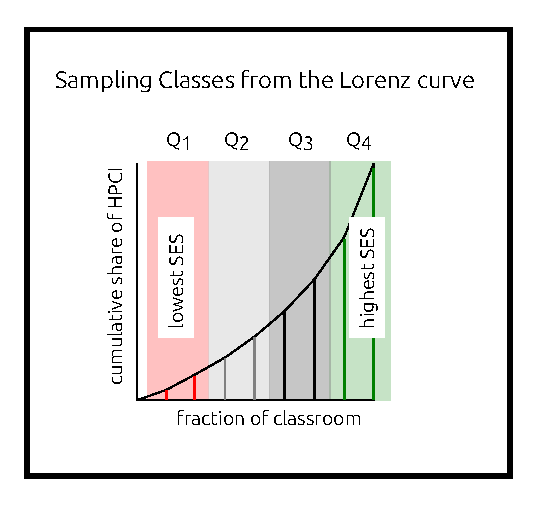
\includegraphics[width=0.9\textwidth]{images/chapter-06/sampling-classes.pdf}}

\par\medskip\ABNTEXfontereduzida\selectfont\textbf{Source:} Created by the author (2024).
\end{figure}